\chapter{Solutions}

Maintenant que la problématique a été établie le but était de définir les caractéristiques clés de notre problème.


\section{Caractéristiques du problème}
Notre agent assistant devra implémenter un système de dialogues avec l'utilisateur répondant aux critères suivants :
\begin{itemize}
	\item le dialogue doit permettre de réunir un ensemble d'informations (heure, jour);
 	\item l'ordre des informations recueillies n'est pas défini (on peut donner l'heure avant le jour, ou le contraire);
 	\item l'entrée de l'utilisateur est textuelle ou bien vocale et en langage naturel ;
 	\item la réponse fournie par l'agent est elle aussi textuelle ou vocale ;
 	\item la mise en place est rapide, réalisable dans un projet de type \og \textit{Proof of Concept} \fg.
\end{itemize}

\section{Solutions scientifiques existantes}
Notre problématique générale est donc d'implémenter un système de dialogue. Plusieurs solutions existent pour ce genre de problème et nous avons donc étudié les plus répandues pour choisir celle (ou celles) qui serait la plus adéquate à notre problème.

\subsection{Analyse syntaxique}
Un analyseur syntaxique pourrait être utilisé pour notre projet. Le principe de cette solution serait de mettre en évidence la structure du texte envoyé par l'utilisateur. Ainsi l'analyseur pourrait savoir quel est le verbe de la phrase, les compléments d'objets, le sujet etc... 

Il retournerait alors un arbre syntaxique (figures \ref{arbre-syntaxique} et \ref{arbre-syntaxique2}). 

~\\\indent Par exemple pour notre projet, si dans l'arbre syntaxique le verbe est \og \textit{mettre} \fg{} et que le complément d'objet est \og \textit{réveil} \fg, l'agent \og comprend \fg{} qu'il doit programmer un réveil. Il va donc continuer le dialogue dans ce sens en demandant l'heure et le jour où le réveil doit être programmé si ces informations lui manquent.

\begin{figure}[!h]
    \centering
    \begin{minipage}{.5\textwidth}
        \centering
        %www.linguistes.com
        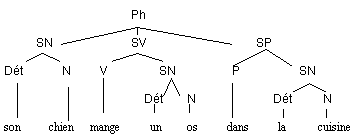
\includegraphics[width=0.9\textwidth]{images/arbre.png}
        \caption{Exemple d'arbre syntaxique}
        \label{arbre-syntaxique}
    \end{minipage}%
    \begin{minipage}{0.5\textwidth}
        \centering
        %http://french.chass.utoronto.ca/
        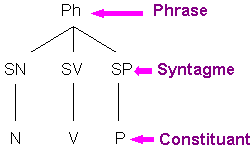
\includegraphics[width=0.9\linewidth]{images/arbre2.png}
        \caption{Hiérarchie de l'arbre syntaxique}
        \label{arbre-syntaxique2}
    \end{minipage}
\end{figure}

~\\\indent
Cette solution pourrait sans doute être implémentée pour notre problème. Mais cela ne résoudrait qu'une partie du problème. En effet il resterait toujours à trouver une solution pour stocker les informations utiles à notre problème comme l'heure et le jour du réveil. 

De plus cette solution semble difficile à implémenter de manière rapide pour un projet de type \og \emph{Proof of Concept} \fg.  

\FloatBarrier

\subsection{Le dialogue par formulaire}
Le dialogue par formulaire est une technique de gestion de dialogue qui permet à l'agent assistant de récolter des informations \emph{via} un dialogue avec l'utilisateur (pour notre projet : alarme, heure et jour). 

Il pourra enregistrer dans différents champs de son formulaire les informations récoltées. Il pourra ensuite envoyer les données du formulaire à un module de traitement qui effectuera des actions en conséquence de ces données.

\begin{figure}[H]
\centering
    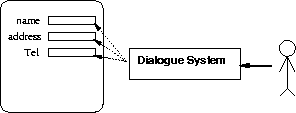
\includegraphics[scale=0.7]{images/slot.png} %www.dfki.de
    \caption{Principe du dialogue par formulaire}
\end{figure}

Cette solution serait très avantageuse pour notre projet. 

En effet, elle répond à tous les critères énoncés précédemment : 
\begin{itemize}
    \item elle permet de réunir des informations (ici dans un formulaire) ;
    \item l'ordre des informations n'est pas défini ;
    \item l'entrée de l'utilisateur est en langage naturel ainsi que la réponse de l'agent ;
    \item la mise en place peut sembler être assez longue mais une application en ligne \textit{DialogFlow} permet de faciliter ceci et rendre l'implémentation d'un dialogue par formulaire beaucoup plus rapide.
\end{itemize}



